%%%%%%%%%%%%%%%%%%%%%%%%%%%%%%%%%%%%%%%%%%%%%%%%%%%%%%%%%%%%%%%%%%%%%%%%%%%%%%%%%%%%%%%%%%%%%%%%%%%

%% document class
%\documentclass{beamer}
%\documentclass[aspectratio=169]{beamer}
\documentclass[handout]{beamer}

%% packages
\usepackage{multimedia}

%% page settings
%% Theme
\usetheme{Berkeley} % theme for slides
%\usetheme{Frankfurt}
%\usetheme{Madrid}

%% Colors
%\usecolortheme{rose} % color for slides
\usecolortheme{default}
%\definecolor{c1}{rgb}{0,0.7,0.6} % some green
%\definecolor{c2}{rgb}{0.9,0.9,0.9} % some gray
%% see http://www.sharelatex.com/learn/Beamer
%\setbeamercolor*{palette primary}{fg=white,bg=c1} % upper part
%\setbeamercolor*{palette secondary}{bg=c2} % left part (background)
%\setbeamercolor*{sidebar left}{fg=white,bg=c1} % left part with links
%\setbeamerfont{section number projected}{ % section numbers
%  family=\rmfamily,
%  series=\bfseries,
%  size=\normalsize
%  }
%\setbeamercolor{section number projected}{bg=c1} % color of section numbers and others (fg: Fontm, bg:Hintergrund)
%\setbeamercolor{item projected}{bg=c1}
%\setbeamercolor{itemize item}{fg=c1}
%\setbeamercolor{author in sidebar}{fg=white}
%\setbeamercolor{footlinecolor}{fg=black,bg=c2}

%% Fonts
\usefonttheme{professionalfonts} % changes fonts

%% Foot
\usenavigationsymbolstemplate{} % deafult controls off
\setbeamertemplate{footline}[frame number] % slide number at the bottom
%\setbeamertemplate{footline}
%{%
%	\leavevmode%
%	\hbox{%
%	\begin{beamercolorbox}[wd=.3\paperwidth,ht=5ex,dp=1.5ex,left,leftskip=2mm]{footlinecolor}%
%		Foot information on the left over several lines
%	\end{beamercolorbox}%
%	\begin{beamercolorbox}[wd=.5\paperwidth,ht=5ex,dp=1.5ex,left,leftskip=2mm]{footlinecolor}%
%		Next foot part
%	\end{beamercolorbox}%
%	\begin{beamercolorbox}[wd=.2\paperwidth,ht=5ex,dp=1.5ex,right,rightskip=2mm]{footlinecolor}%
%		\insertframenumber{} / \inserttotalframenumber%
%	\end{beamercolorbox}%
%	}%
%	\vskip0pt%
%}

%% new commands
\newcommand{\cm}[1]{{\tt \textcolor{orange}{#1}}}
\newcommand{\wl}[2]{\href{#2}{\textcolor{blue}{#1}}}
\newcommand{\att}[2]{\href{#2}{\textcolor{blue}{#1}}}

%%%%%%%%%%%%%%%%%%%%%%%%%%%%%%%%%%%%%%%%%%%%%%%%%%%%%%%%%%%%%%%%%%%%%%%%%%%%%%%%%%%%%%%%%%%%%%%%%%%

\begin{document}

%%%%%%%%%%%%%%%%%%%%%%%%%%%%%%%%%%%%%%%%%%%%%%%%%%%%%%%%%%%%%%%%%%%%%%%%%%%%%%%%%%%%%%%%%%%%%%%%%%%
%%%%%%%%%%%%%%%%%%%%%%%%%%%%%%%%%%%%%%%%%%%%%%%%%%%%%%%%%%%%%%%%%%%%%%%%%%%%%%%%%%%%%%%%%%%%%%%%%%%
%%%%%%%%%%%%%%%%%%%%%%%%%%%%%%%%%%%%%%%%%%%%%%%%%%%%%%%%%%%%%%%%%%%%%%%%%%%%%%%%%%%%%%%%%%%%%%%%%%%

\author[Mauricio]{Mauricio Lobos}
\title[Basic elements]{Basic elements for a presentation using \LaTeX{}}
\titlegraphic{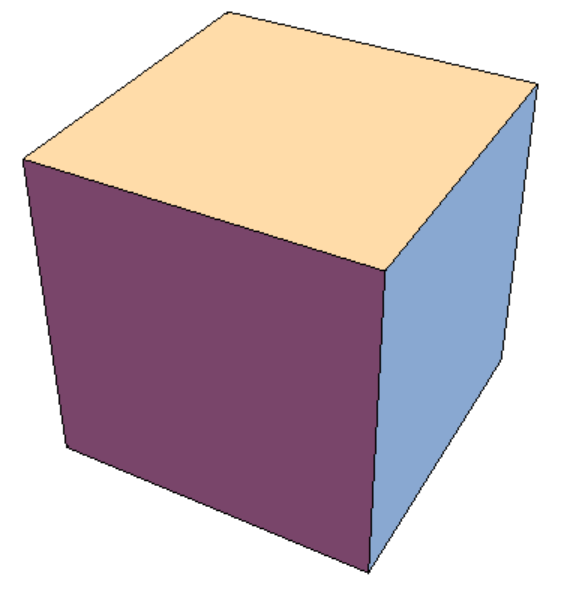
\includegraphics[width=0.2\textwidth]{figures/cube}}
\institute{Wherever you work}
\date{City, date}
\frame{\titlepage}

%%%%%%%%%%%%%%%%%%%%%%%%%%%%%%%%%%%%%%%%%%%%%%%%%%%%%%%%%%%%%%%%%%%%%%%%%%%%%%%%%%%%%%%%%%%%%%%%%%%

\begin{frame}{Table of contents}
\tableofcontents
%\tableofcontents[hideallsubsections]
\end{frame}

%%%%%%%%%%%%%%%%%%%%%%%%%%%%%%%%%%%%%%%%%%%%%%%%%%%%%%%%%%%%%%%%%%%%%%%%%%%%%%%%%%%%%%%%%%%%%%%%%%%
%%%%%%%%%%%%%%%%%%%%%%%%%%%%%%%%%%%%%%%%%%%%%%%%%%%%%%%%%%%%%%%%%%%%%%%%%%%%%%%%%%%%%%%%%%%%%%%%%%%

\section{First settings}

\begin{frame}{Table of contents}
\tableofcontents[currentsection,hidesubsections]
\end{frame}

%%%%%%%%%%%%%%%%%%%%%%%%%%%%%%%%%%%%%%%%%%%%%%%%%%%%%%%%%%%%%%%%%%%%%%%%%%%%%%%%%%%%%%%%%%%%%%%%%%%

\subsection[Themes]{Themes, colors and fonts}

\begin{frame}{Themes, colors and fonts}
\begin{itemize}
	\item 
		Themes can be changed with the command \cm{usetheme}. \pause 
		A list of the different themes can be found \wl{here}{http://deic.uab.es/~iblanes/beamer_gallery/index_by_theme.html}. \pause
	\item 
		The colors of a theme can be changed with the command \cm{usecolortheme}. \pause
		A list of the different colors can be found \wl{here}{http://deic.uab.es/~iblanes/beamer_gallery/index_by_color.html}. \pause
	\item 
		The fonts can be changed with the command \cm{usefonttheme}. \pause
		A list of the different fonts can be found here \wl{here}{http://deic.uab.es/~iblanes/beamer_gallery/index_by_font.html}. \pause
\end{itemize}
See the difference in this equation
\begin{equation}
	f(x) = x^{2345}\sin(x) .
\end{equation}
\end{frame}


\begin{frame}{Custom colors}
You can also define your own colors with the commands \cm{definecolor} and \cm{setbeamercolor}.
\end{frame}

%%%%%%%%%%%%%%%%%%%%%%%%%%%%%%%%%%%%%%%%%%%%%%%%%%%%%%%%%%%%%%%%%%%%%%%%%%%%%%%%%%%%%%%%%%%%%%%%%%%

\subsection[Frame numbers]{Frame numeration and foot}

\begin{frame}{Frame number}
The frame number can be added to the bottom of the slide with the command \cm{setbeamertemplate\{footline\}[frame number]}.
\end{frame}


\begin{frame}{Foot}
Alternative the foot of the presentation can be changed with further options for \cm{setbeamertemplate\{footline\}}.
\end{frame}

%%%%%%%%%%%%%%%%%%%%%%%%%%%%%%%%%%%%%%%%%%%%%%%%%%%%%%%%%%%%%%%%%%%%%%%%%%%%%%%%%%%%%%%%%%%%%%%%%%%

\subsection[Aspect]{Aspect ratio}

\begin{frame}{Aspect ratio}
With \cm{documentclass[aspectratio=169]\{beamer\}} you will create slides in 16:9 format.
\end{frame}

%%%%%%%%%%%%%%%%%%%%%%%%%%%%%%%%%%%%%%%%%%%%%%%%%%%%%%%%%%%%%%%%%%%%%%%%%%%%%%%%%%%%%%%%%%%%%%%%%%%
%%%%%%%%%%%%%%%%%%%%%%%%%%%%%%%%%%%%%%%%%%%%%%%%%%%%%%%%%%%%%%%%%%%%%%%%%%%%%%%%%%%%%%%%%%%%%%%%%%%

\section[Elements]{Presentation elements}

\begin{frame}{Table of contents}
\tableofcontents[currentsection,hidesubsections]
\end{frame}

%%%%%%%%%%%%%%%%%%%%%%%%%%%%%%%%%%%%%%%%%%%%%%%%%%%%%%%%%%%%%%%%%%%%%%%%%%%%%%%%%%%%%%%%%%%%%%%%%%%

\subsection{Highlight current section}
\begin{frame}{Where are we?}
Although most of the themes have a sidebar with the sections of the presentation, it is still for some people very useful to highlight the upcoming section and its contents. \pause
This can be achieved using the command \cm{tableofcontents[currentsection]} just after the section definition.
\end{frame}

%%%%%%%%%%%%%%%%%%%%%%%%%%%%%%%%%%%%%%%%%%%%%%%%%%%%%%%%%%%%%%%%%%%%%%%%%%%%%%%%%%%%%%%%%%%%%%%%%%%

\subsection{Columns}
\begin{frame}{Columns}
Columns can be used in order to separate content. \\[1cm]
\begin{columns}[t]
\column{0.45\textwidth}
	Some text in the first column. It is important to see here that the content in the columns are aligned to the top. You can choose t,c or b.
\column{0.45\textwidth}
	Some text the second column.
\end{columns}
\end{frame}

%%%%%%%%%%%%%%%%%%%%%%%%%%%%%%%%%%%%%%%%%%%%%%%%%%%%%%%%%%%%%%%%%%%%%%%%%%%%%%%%%%%%%%%%%%%%%%%%%%%

\subsection{Images, videos and attachments}
\begin{frame}{Embedding images}
You may want to use different kind of images like PNG and EPS figures. In order to be able to work with EPS figures you need to adapt your compilation procedure. Here you can see a PNG figure.
\begin{center}
	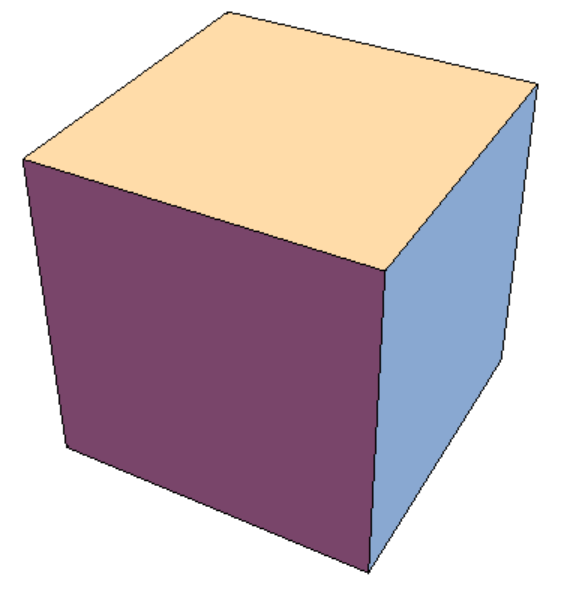
\includegraphics[width=0.2\textwidth]{figures/cube}
\end{center}
For conversion of PNG figures into EPS search in Google for a converter or go \wl{here}{http://www.tlhiv.org/rast2vec/}.
\end{frame}


\begin{frame}{Setting a link to a video}
You are also able to link videos to the created PDF using the command \cm{movie}.
\begin{center}
	\movie[externalviewer]{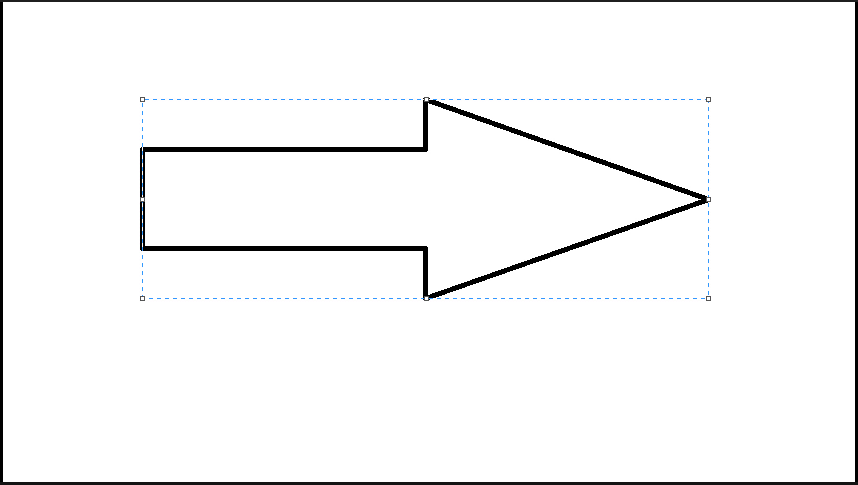
\includegraphics[width=3cm]{figures/arrow}}{videos/exmp4.mp4}
	\qquad
	\movie[externalviewer]{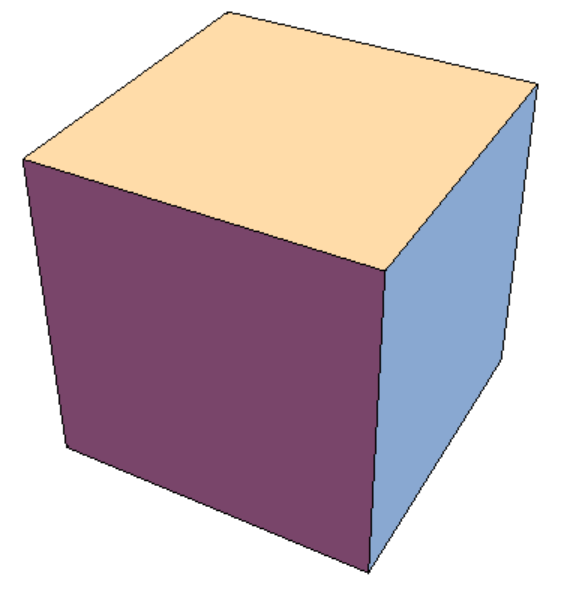
\includegraphics[width=2cm]{figures/cube}}{videos/exavi.avi} \\[0.3cm]
	\movie[externalviewer]{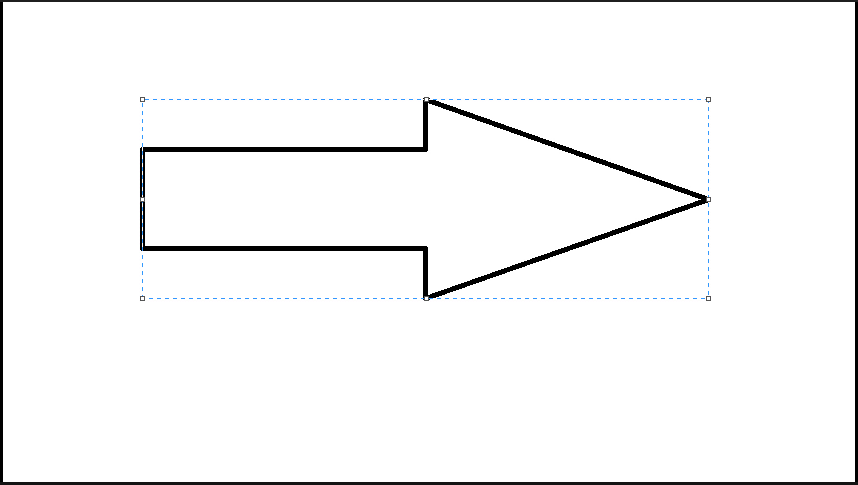
\includegraphics[width=3cm]{figures/arrow}}{videos/exmp4.mp4}
	\qquad
	\movie[externalviewer]{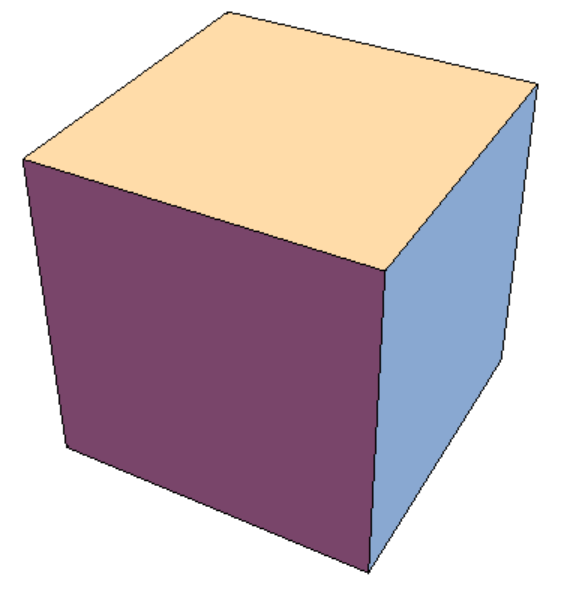
\includegraphics[width=2cm]{figures/cube}}{videos/exavimp4.mp4}
\end{center}
A fantastic explanation on how to convert videos with the completely free VLC player can be found \wl{here}{http://www.tweakandtrick.com/2014/01/convert-videos-vlc.html}.
\end{frame}


\begin{frame}{Other attachments}
You might also want to show other attached files, e.g., \att{manipulate}{run:attachments/manipulate.nb}.
\end{frame}

%%%%%%%%%%%%%%%%%%%%%%%%%%%%%%%%%%%%%%%%%%%%%%%%%%%%%%%%%%%%%%%%%%%%%%%%%%%%%%%%%%%%%%%%%%%%%%%%%%%

\subsection{Overlays: pause, visible, unconver, only}
\begin{frame}{Overlays: pause}
An itemized or enumerated list can be paused at several parts using the command \cm{pause}, e.g.
\begin{itemize}
	\pause
	\item first
	\pause
	\item second
	\pause
	\item third
	\item fourth
\end{itemize}
\end{frame}

\begin{frame}{Overlays: visible, unconver and only}
If a more elaborated form has to be presented, use unconver and only. Example: \\[0.3cm]

\begin{columns}[t]
\column{0.45\textwidth}
	Description of some concept \\
	\visible<2->{
	\begin{enumerate}
	\item	
		Point 1
	\visible<3->{
	\item
		Point 2
	\item
		Point 3
	\visible<5->{
	\item
		Point 4
	}
	}
	\end{enumerate}	
	}
\column{0.5\textwidth}
	\mbox{} \\
	\begin{overlayarea}{\textwidth}{0.4\textheight}
	\only<4-5>{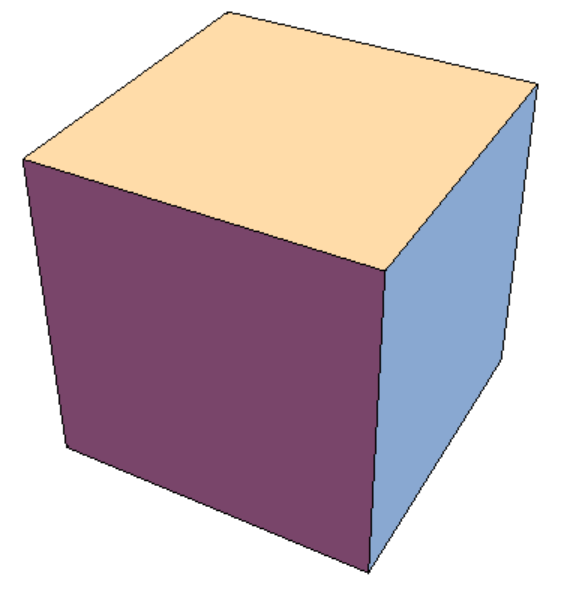
\includegraphics[width=0.4\textwidth]{figures/cube}}
	\only<6->{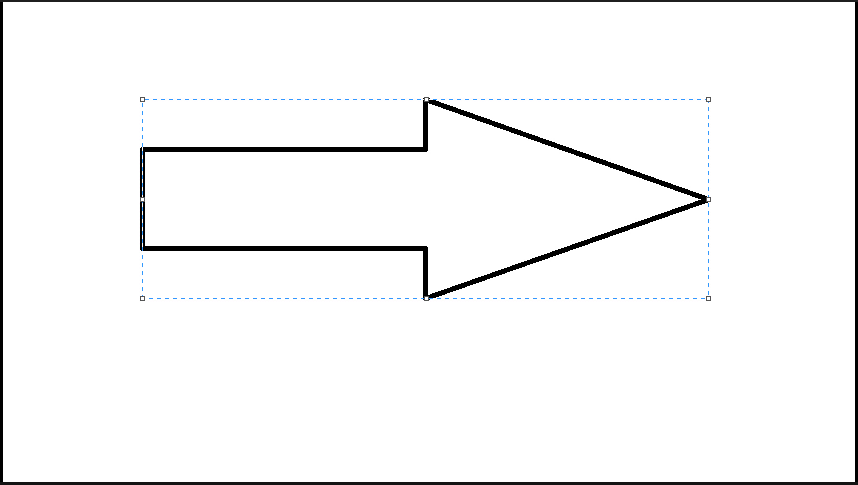
\includegraphics[width=0.9\textwidth]{figures/arrow}}
	\end{overlayarea}
	More Text.
\end{columns}

\end{frame}

%%%%%%%%%%%%%%%%%%%%%%%%%%%%%%%%%%%%%%%%%%%%%%%%%%%%%%%%%%%%%%%%%%%%%%%%%%%%%%%%%%%%%%%%%%%%%%%%%%%

\subsection{Tables}
\begin{frame}{Presentation of data}
As in the other \LaTeX{} documents you can also use here tables in order to present data.
\begin{center}
	\begin{tabular}{l|ccr}
	\hline\hline	
	 & bla & ble & bli \\ \hline
	first
		& sdfajfdlkö
		& sdjdklf
		& djk \\
	second
		& sfd
		& fdgdfgds
		& dfgshgsdfh \\ \hline\hline
	\end{tabular}
\end{center}
\end{frame}

%%%%%%%%%%%%%%%%%%%%%%%%%%%%%%%%%%%%%%%%%%%%%%%%%%%%%%%%%%%%%%%%%%%%%%%%%%%%%%%%%%%%%%%%%%%%%%%%%%%

\subsection[Blocks]{Text blocks, definitions, theorems and proofs}

\begin{frame}{Text blocks}
You have the possibility to use the environment \cm{block} for separating important content and concepts from the rest of the text. \pause
\begin{block}{Title of the concept}
	Description of the concept comes in this region. You are able to define more stuff in this region, e.g. equations
	\begin{equation}
		a + b = c
	\end{equation}
	and more.
\end{block}
\end{frame}

\begin{frame}{Text blocks}
More blocks \pause
\begin{definition}[Name]
	Description
\end{definition}
\pause
\begin{theorem}[Name]
	Description
\end{theorem}
\pause
\begin{proof}
	Proof
\end{proof}
\end{frame}

%%%%%%%%%%%%%%%%%%%%%%%%%%%%%%%%%%%%%%%%%%%%%%%%%%%%%%%%%%%%%%%%%%%%%%%%%%%%%%%%%%%%%%%%%%%%%%%%%%%

\subsection[Math]{Mathematical content}
\begin{frame}{Mathematical content}
Of course you are able to create also equations
\begin{equation}
	m \ddot{x} = \sum_{i=1}^n F_i \quad , \quad
	\delta H = 0 \quad , \quad
	x(t) = \int_0^t\limits{ v(s) }ds
\end{equation}
separately or in the text $f(x)=x^2$ using the common commands.
\end{frame}

%%%%%%%%%%%%%%%%%%%%%%%%%%%%%%%%%%%%%%%%%%%%%%%%%%%%%%%%%%%%%%%%%%%%%%%%%%%%%%%%%%%%%%%%%%%%%%%%%%%
%%%%%%%%%%%%%%%%%%%%%%%%%%%%%%%%%%%%%%%%%%%%%%%%%%%%%%%%%%%%%%%%%%%%%%%%%%%%%%%%%%%%%%%%%%%%%%%%%%%

\section[Handout]{Presentation handout}

\begin{frame}{Table of contents}
\tableofcontents[currentsection,hidesubsections]
\end{frame}

%%%%%%%%%%%%%%%%%%%%%%%%%%%%%%%%%%%%%%%%%%%%%%%%%%%%%%%%%%%%%%%%%%%%%%%%%%%%%%%%%%%%%%%%%%%%%%%%%%%

\subsection{Handout option}
\begin{frame}{How to create a handout?}
As you could see using the command pause a lot of PDF pages are created. May be you will want to give an handout of your presentation without the pauses. This can be done with the document class option \cm{handout}. This will then ignore all pauses and a "reduced" PDF will be created.
\end{frame}

%%%%%%%%%%%%%%%%%%%%%%%%%%%%%%%%%%%%%%%%%%%%%%%%%%%%%%%%%%%%%%%%%%%%%%%%%%%%%%%%%%%%%%%%%%%%%%%%%%%
%%%%%%%%%%%%%%%%%%%%%%%%%%%%%%%%%%%%%%%%%%%%%%%%%%%%%%%%%%%%%%%%%%%%%%%%%%%%%%%%%%%%%%%%%%%%%%%%%%%

\end{document}

%%%%%%%%%%%%%%%%%%%%%%%%%%%%%%%%%%%%%%%%%%%%%%%%%%%%%%%%%%%%%%%%%%%%%%%%%%%%%%%%%%%%%%%%%%%%%%%%%%%
%%%%%%%%%%%%%%%%%%%%%%%%%%%%%%%%%%%%%%%%%%%%%%%%%%%%%%%%%%%%%%%%%%%%%%%%%%%%%%%%%%%%%%%%%%%%%%%%%%%
%%%%%%%%%%%%%%%%%%%%%%%%%%%%%%%%%%%%%%%%%%%%%%%%%%%%%%%%%%%%%%%%%%%%%%%%%%%%%%%%%%%%%%%%%%%%%%%%%%%
